\chapter{Method} \label{chap:method}
In this work tow methods combining state of the art techniques have been proposed. A full description is delineated in this Chapter.

\section{Preprocessing}\label{sec:preproces}

Given that the background information is not needed in any of the two proposed methods, it is required to first detect the faces from the images and second align all of them (Figure \ref{fig:preprocessing}).

\textbf{Face detection} was performed using the Viola Jones algorithm from the open source library OpenCV \cite{opencv_library}. An heuristic method was used to detect faces. Given that each images of the database contains a single face the detection algorithm should choose among all the detected faces. A Haar Cascade classifier was trained with nearly 5000 face images from different mugshot databases and more than 9500 negative samples. This classifier plus the standard frontal and lateral OpenCV cascade classifiers were used to detect faces in the images. Then an eye cascade classifier was used among the detected faces to drop out the ones where no eyes were detected. Finally, the biggest detected face is selected. After detecting the face, the image is cropped and resized into a $200 \times 200$.

\textbf{Face alignment}, 68 facial landmarks were extracted for every detected face with a version of the algorithm proposed by Shaoqing Ren et al. \cite{ren2014face}. The algorithm was trained with almost 5000 face labelled images from FG-NET, AFW, HELEN, IBUG and LFPW face databases. After extracting all the landmarks all the faces are aligned.

All the images where transformed into \textbf{grey scale} because of the variation of the data in terms of colour (some images are in grey scale other in RGB).

\begin{figure}[!h]
	\centering
	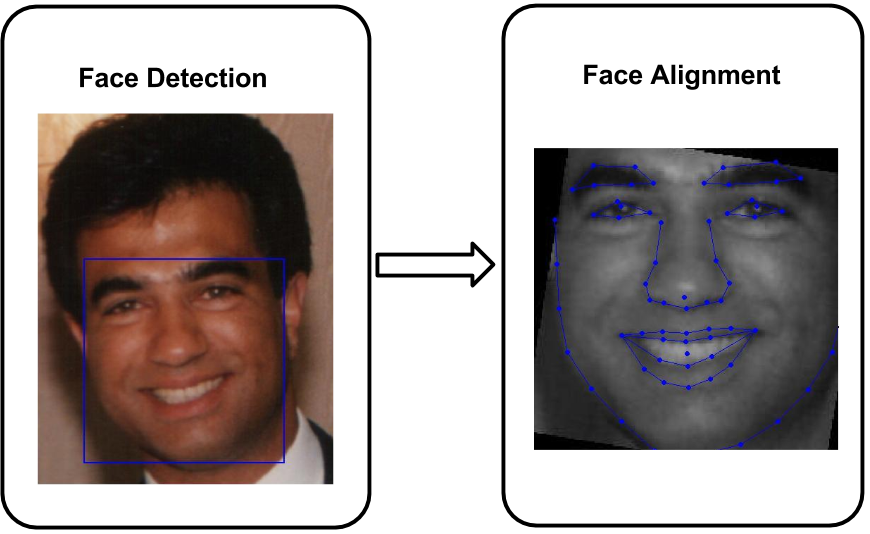
\includegraphics[width=\textwidth]{figures/preprocessing}
	\caption{Face Detection and Face Alignment.}
	\label{fig:preprocessing}
\end{figure}


\section{Biologically Inspired Method}\label{sec:BIF}
As mentioned in Section \ref{subsec:BIF} \acrfull{bif} have been proven to work specially good in age estimation \cite{conf/cvpr/GuoMFH09}\cite{han:age}. In this work a method is proposed using \gls{bif} as age representation and a hierarchical framework with \gls{svm} and \gls{svr} as a learning method.
 
\subsection{Background}

Inspired by how the visual cortex works, Maximilian Riesenhuber and Tomaso Poggio \cite{Riesenhuber99hierarchicalmodels} proposed the \gls{bif} model for object recognition called ``HMAX'' based on the hierarchical model of the visual nervous system proposed by D. H. Hubel and T. N. Wiesel \cite{Hubel:62}. 

The ``HMAX'' model is composed by layers that will contain increasingly sophisticated representations. There are two type of layers called simple ($S_1$) and complex ($C_1$). Layer $S_1$ consists a battery of Gabor filters with different orientation and scales and layer $C_1$ is a pooling layer, in this model is a ``MAX'' pooling layer. There are many variations and extensions of this model made by many authors, Serre et al. \cite{4069258}\cite{1467551} introducing two more layers $S_2$ and $C_2$ or Mayers and Wolf \cite{Meyers:2008:UBI:1325290.1325298} uses a spacial $S_2$ layer called $S_2$ facial features (S2FF) for face recognition.

\begin{table}[!h]
	\centering
	\begin{tabular}{|M{2cm}|M{2cm}|M{1.5cm}||c|c|c|}
		\hline
		\multicolumn{3}{|c||}{\textbf{$C_1$ layer}}                                               & \multicolumn{3}{c|}{\textbf{$S_1$ layer}}                \\ \hline
		Scale Band $S$    & Pool grid $(q\times q)$    & Overlap $\Delta n$     & Filter size $n$  & Gabor $\sigma$ & Gabor $\lambda$ \\ \hhline{===#===}
		\multirow{2}{*}{Band 1} & \multirow{2}{*}{$6 \times 6$}   & \multirow{2}{*}{3}  & $5 \times 5$   & 2.0            & 2.5           \\
		&                                 &                     & $7 \times 7$   & 2.8            & 3.5           \\ \hline
		\multirow{2}{*}{Band 2} & \multirow{2}{*}{$8 \times 8$}   & \multirow{2}{*}{4}  & $9 \times 9$   & 3.6            & 4.6           \\
		&                                 &                     & $11 \times 11$ & 4.5            & 5.6           \\ \hline
		\multirow{2}{*}{Band 3} & \multirow{2}{*}{$10 \times 10$} & \multirow{2}{*}{5}  & $13 \times 13$ & 5.4            & 6.8           \\
		&                                 &                     & $15 \times 15$ & 6.3            & 7.9           \\ \hline
		\multirow{2}{*}{Band 4} & \multirow{2}{*}{$12 \times 12$} & \multirow{2}{*}{6}  & $17 \times 17$ & 7.3            & 9.1           \\
		&                                 &                     & $19 \times 19$ & 8.2            & 10.3          \\ \hline
		\multirow{2}{*}{Band 5} & \multirow{2}{*}{$14 \times 14$} & \multirow{2}{*}{7}  & $21 \times 21$ & 9.2            & 11.5          \\
		&                                 &                     & $23 \times 23$ & 10.2           & 12.7          \\ \hline
		\multirow{2}{*}{Band 6} & \multirow{2}{*}{$16 \times 16$} & \multirow{2}{*}{8}  & $25 \times 25$ & 11.3           & 14.1          \\
		&                                 &                     & $27 \times 27$ & 12.3           & 15.4          \\ \hline
		\multirow{2}{*}{Band 7} & \multirow{2}{*}{$18 \times 18$} & \multirow{2}{*}{9}  & $29 \times 29$ & 13.4           & 16.8          \\
		&                                 &                     & $31 \times 31$ & 14.6           & 18.2          \\ \hline
		\multirow{2}{*}{Band 8} & \multirow{2}{*}{$20 \times 20$} & \multirow{2}{*}{10} & $33 \times 33$ & 15.8           & 19.7          \\
		&                                 &                     & $35 \times 35$ & 17.0           & 21.2          \\ \hline
	\end{tabular}
	\caption{$S_1$ and $C_1$ parameters.}
	\label{tab:bif_param}
\end{table}

The proposed method in this work used the \gls{bif} model described by Guo et al. \cite{conf/cvpr/GuoMFH09} that uses ``STD'' pool operator instead of ``MAX'' operator (Figure \ref{fig:bif}). 

\begin{figure}[!h]
	\centering
	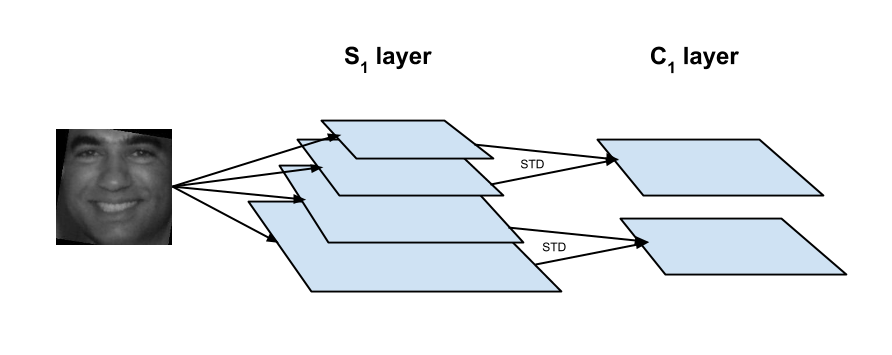
\includegraphics[width=\textwidth]{figures/BIF}
	\caption{\acrfull{bif}.}
	\label{fig:bif}
\end{figure}


\textbf{$S_1$ layer} is formed by $S_1$ units which take as input a grey image of size $200\times 200$. These units are usually modelled by Gabor filters, given $(x,y)$ pixel coordinates of the input image,

\begin{equation}
G(x,y) = exp\bigg(-\frac{X^2+\gamma^2 Y^2}{2\sigma^2}\bigg)\cdot cos(\frac{2\pi}{\lambda}X)\ ,
\end{equation}

where $X=x\cos\theta + y\sin\theta$ and $Y = -x\sin\theta + y\cos\theta$ are the rotations of the filter with angle $\theta\in[0,\pi]$. The aspect ration $\gamma$ is set to $0.3$, the width $\sigma$, the wavelength $\lambda$ and the filter sizes $n$ are adjusted as in Table \ref{tab:bif_param}. These parameters are empirically determined based on reactions of the visual cortex to real stimuli \cite{4069258}. 

\textbf{$C_1$ layer} is formed by $C_1$ units which pool over the $S_1$ units with the same orientation and from the same scale band (see Table \ref{tab:bif_param}). Each scale band $S$ contains two adjacent filter sizes, for instance, scale band 1 contains filter with sizes $5\times5$ and $7\times7$. The scale band also determines the sizes of the neighbourhood over which the $C_1$ units pool ($q\times q$). The pooling operator used in this method is the ``STD'' operator proposed by Guo et al. \cite{conf/cvpr/GuoMFH09},

\begin{equation}
std_{j,j+1} = \sqrt{\frac{1}{q\times q}\sum_{i=1}^{q\times q}(F_i - \bar{F})^2} \ ,
\end{equation}

where $F_i$ is the maximum value of two consecutive $S_1$ units output in the same scale band at pixel index $i$, 

\begin{equation}
F_i = \max(x_i^j,x_i^{j+1})\ ,
\end{equation}

where $x_i^j$ and $x_i^{j+1}$ are the filtered values with scales $j$ and $j+1$ at position $i$. $\bar{F}$ is the mean of the filtered values in the neighbourhood $q\times q$.

The $C_1$ units are concatenated into a single feature vector for each input image.


\subsection{System overview}

This method combines a hierarchical framework and a hybrid face model, mixing \gls{bif} features and face shape landmarks to optimize the performance. The pipeline consists of three steps (see Figure \ref{fig:pipeline}).

\begin{figure}[!h]
	\centering
	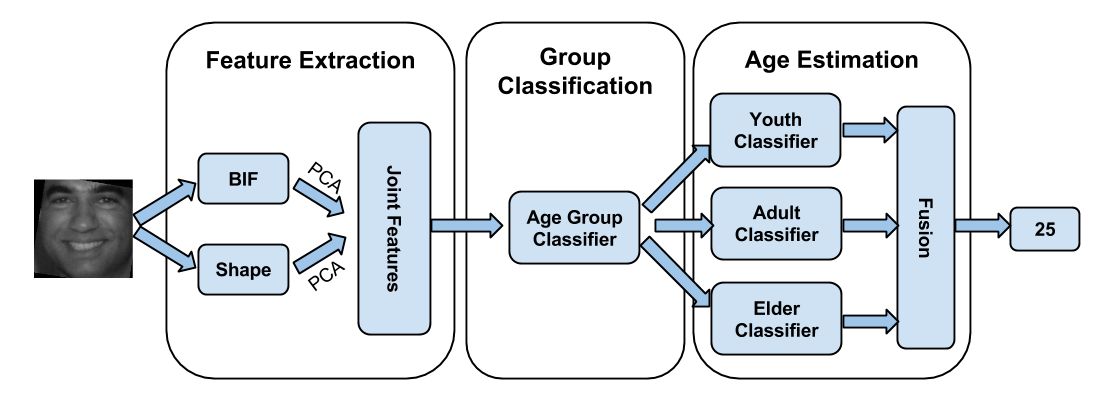
\includegraphics[width=\textwidth]{figures/pipeline}
	\caption{Biologically Inspired Method Pipeline.}
	\label{fig:pipeline}
\end{figure}

\textbf{Feature extraction}: 
After the face alignment is done, \gls{bif} features are extracted from each face image as described above. Because of the high dimensionality of the data ($\sim3000$ \gls{bif} features and 138 shape landmark coordinates) feature reduction is needed. \gls{pca} is used to reduce dimensionality of both shape and \gls{bif}. As shows Figure \ref{fig:pipeline} \gls{bif} and shape features are concatenated into a single feature vector.

\textbf{Age Group Classification}:
In this stage the images are classified into three age groups with age ranges (0-18), (19-45) and (45-100). The classifier used is a linear \gls{svm} as suggested in \cite{4531189}.

\textbf{Age Estimation}:
Three \gls{svr} with \gls{rbf} kernel were trained to perform age regression in a specific age range. The data used to fit the regressors were images within 5-years-overlap between age ranges to reduce the misclassification error as proposed in \cite{han:age}. 

In order to improve the system performance a last fusion step is done by averaging the two nearest age regressors, i.e. if the age group classifier predicts that a given face belongs to the adult age group (19-45)] and the adult-specific regression function predicts that the exact age is 43, then in the fusion step would average the adult regressor with the elder regressor.


\section{Deep Learning Method}

Deep Learning methods have not been fully explored in the age estimation problem. However, the rise of Deep Learning methods these last few years makes very likely that more works will base their approaches on this technique. In this work a method based on \gls{cnn} is analysed.

\subsection{Background}
\gls{cnn} were first proposed by Kunihiko Fukushima \cite{fukushima:neocognitronbc} in 1980 and then further improved by Y. LeCun et al. \cite{Lecun98gradient-basedlearning} in 1998. This particular type of Neural Network has been widely used in Computer Vision because of the way its ability to capture spacial relations. Some of the most successful applications were seen in the ImageNet Large Scale Visual Recognition Challenge \cite{DBLP:journals/corr/RussakovskyDSKSMHKKBBF14} in 2014 where the winner \cite{DBLP:journals/corr/SzegedyLJSRAEVR14} achieved object detection to $0.439329$, and reduced classification error to $0.06656$ in the ImageNet database which contains millions of images and thousands of classes. Also early this year S. Farfade et al. \cite{DBLP:journals/corr/FarfadeSL15} proposed a method of multi-view face detection using \gls{cnn} achieving a hight accuracy being able to detect faces from an up-side down view or partially occluded.

\begin{figure}[!h]
	\centering
	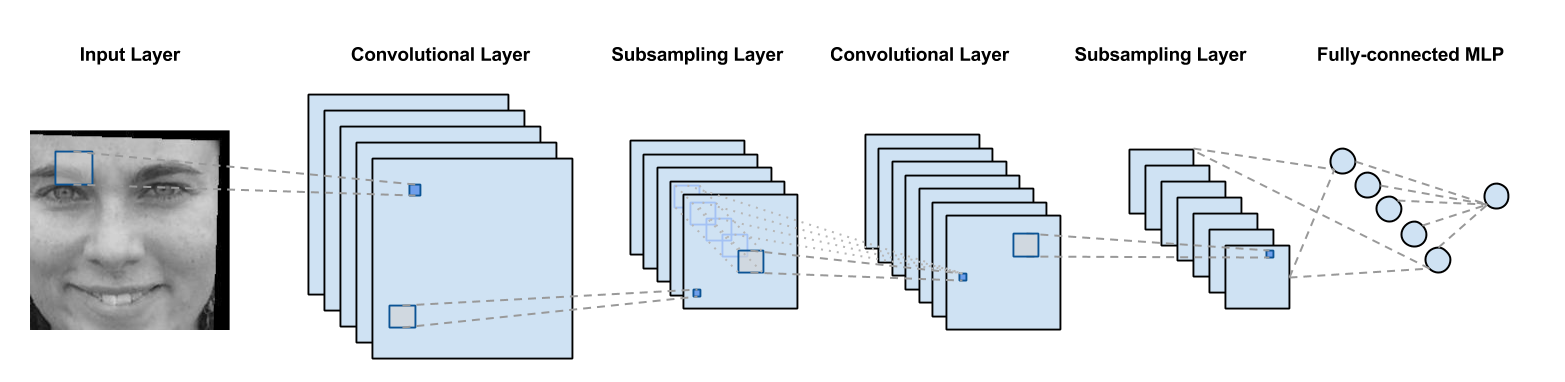
\includegraphics[width=\textwidth]{figures/CNN_sample}
	\caption{Example of Convolutional Neural Network.}
	\label{fig:cnnSample}
\end{figure}

\gls{cnn} consists of a number of convolutional and subsampling layers optionally followed by fully connected layers (see Figure \ref{fig:cnnSample}). The \gls{cnn} input is an image of size $m\times m\times r$. The convolutional layer contains $k$ kernels (filters) of size $n\times n\times q$ where $n \leq m$ and $q \leq r$. The filters will produce $k$ feature maps of size $m - n - 1 $. Each map is then subsampled typically with max or mean pulling over $p\times p$ contiguous region where $p$ is small (typically between 2 and 5).

After the convolutional layers there may be any number of fully connected layers.

\subsection{System overview}

The \gls{cnn} proposed in this work for age estimation is inspired on \cite{yiage} \cite{yan2014}. The network was implemented using the Python library Theano \cite{Bastien-Theano-2012}\cite{bergstra+al:2010-scipy} to optimize the training using the GPU. The proposed network topology is composed by three convolutional layers each of these followed by subsampling pooling layers and three fully connected layers at the end.

More in detail Table \ref{tab:cnnTopo} shows the network topology layer by layer. The pooling layers use all the ``MAX'' operator and the fully-connected layers have ReLu \cite{conf/icml/NairH10} activation function. The proposed \gls{cnn} is designed to do regression returning a single value for each input instance.

\begin{table}[!h]
	\centering
	\begin{tabular}{|l||c|c|c|c|}
		\hline
		\textbf{Layer} & \textbf{Input size} & \textbf{Output size} & \textbf{Filter size} & \textbf{Pooling size} \\ \hhline{=#====}
		
		Conv1 & $200\times 200$ & $190\times190$ & $10*(11\times11)$ & -\\ \hline
		
		Pool1 & $190\times190$ & $95\times95$ & - & $(2,2)$\\ \hline
		
		Conv2 & $95\times95$ & $89\times89$ & $20*(7\times7)$ & - \\ \hline
		
		Pool2 & $89\times89$ & $44\times44$ & - & $(2,2)$\\ \hline
		
		Conv3 & $44\times44$ & $40\times40$ & $40*(5\times5)$ & - \\ \hline
		
		Pool3 & $40\times40$ & $20\times20$ & - & $(2,2)$\\ \hline
		
		Full1 & $16,000$ & $500$ & - & - \\ \hline
		
		Full2 & $500$ & $200$ & - & - \\ \hline
		
		Full3 & $200$ & $1$ & - & - \\ \hline
	\end{tabular}
	\caption{Proposed \gls{cnn} topology.}
	\label{tab:cnnTopo}
\end{table}







